\documentclass[11pt]{article}

\usepackage{fullpage}
\usepackage{graphicx}
\usepackage{amsmath}
\usepackage{amssymb}
\usepackage{amsthm}
\usepackage{fancyvrb}

% useful package
\usepackage[obeyspaces]{url}
\usepackage{listings}  % coding blocks
\usepackage[svgnames]{xcolor}
\graphicspath{ {./pic/} }

% codign block setting
\definecolor{codegreen}{rgb}{0,0.6,0}
\definecolor{codegray}{rgb}{0.5,0.5,0.5}
\definecolor{codepurple}{rgb}{0.58,0,0.82}
\definecolor{backcolour}{rgb}{0.95,0.95,0.92}

\lstdefinestyle{mystyle}{
    backgroundcolor=\color{backcolour},   
    commentstyle=\color{codegreen},
    keywordstyle=\color{magenta},
    numberstyle=\tiny\color{codegray},
    stringstyle=\color{codepurple},
    basicstyle=\ttfamily\footnotesize,
    breakatwhitespace=false,         
    breaklines=true,    captionpos=b,                    
    keepspaces=true, numbers=left,                    
    numbersep=5pt, showspaces=false,                
    showstringspaces=false, showtabs=false, tabsize=2}
\lstset{style=mystyle}


\parindent0in
\pagestyle{plain}
\thispagestyle{plain}


%% UPDATE MACRO DEFINITIONS %%
\newcommand{\myname}{Xiang Jyun, Jhang}
\newcommand{\assignment}{Homework 1}
\newcommand{\duedate}{March 10, 2024}

%% mathematical notation
\newcommand{\ept}{\mathbb{E}}
\newcommand{\normal}{\mathcal{N}}


\begin{document}


\textbf{National Taiwan University}\hfill\textbf{\myname}\\[0.01in]
\textbf{ECON 5211 Labor Economics I}\hfill\textbf{\assignment}\\[0.01in]
\textbf{Prof.\ Kuan Ming, Chen}\hfill\textbf{\duedate}\\
\smallskip\hrule\bigskip



% question 1
\section{Programming Setup}

    % Q1.1
    \subsection{Setup Datacamp}
        
\includegraphics[scale = 0.35]{Q1_1_2_datacamp.png}

    % Q1.2
    \subsection{R}
        For installation process and HelloWorld example, please refer to the file located at \path{"/homework/homework1/R_code"}

    % Q1.3
    \subsection{Debugger}
        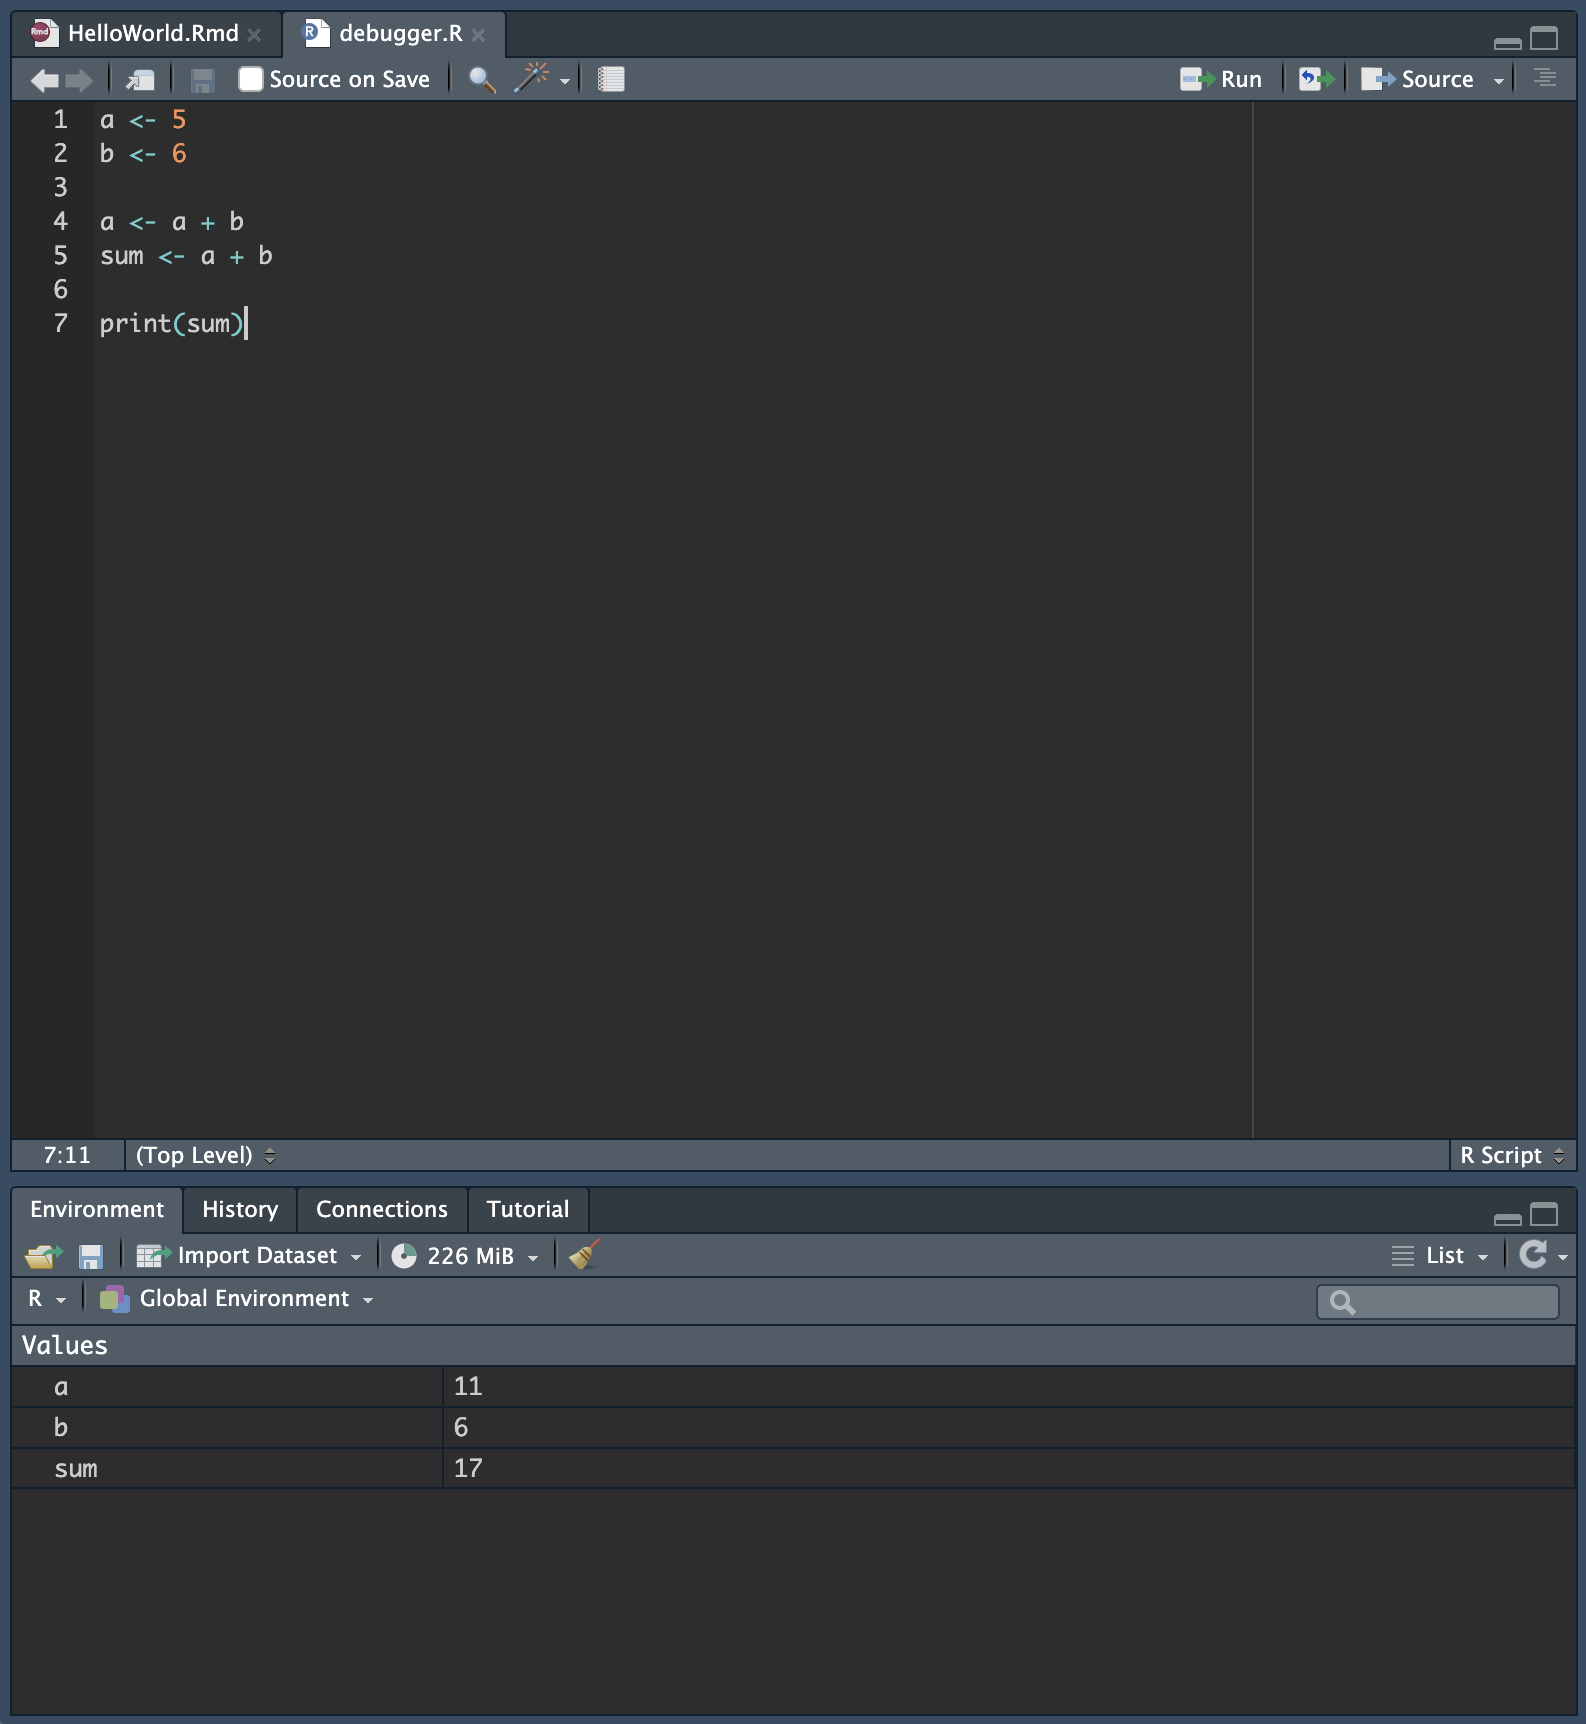
\includegraphics[scale = 0.4]{Q1_3_1_debugger.png} 
        \newline
        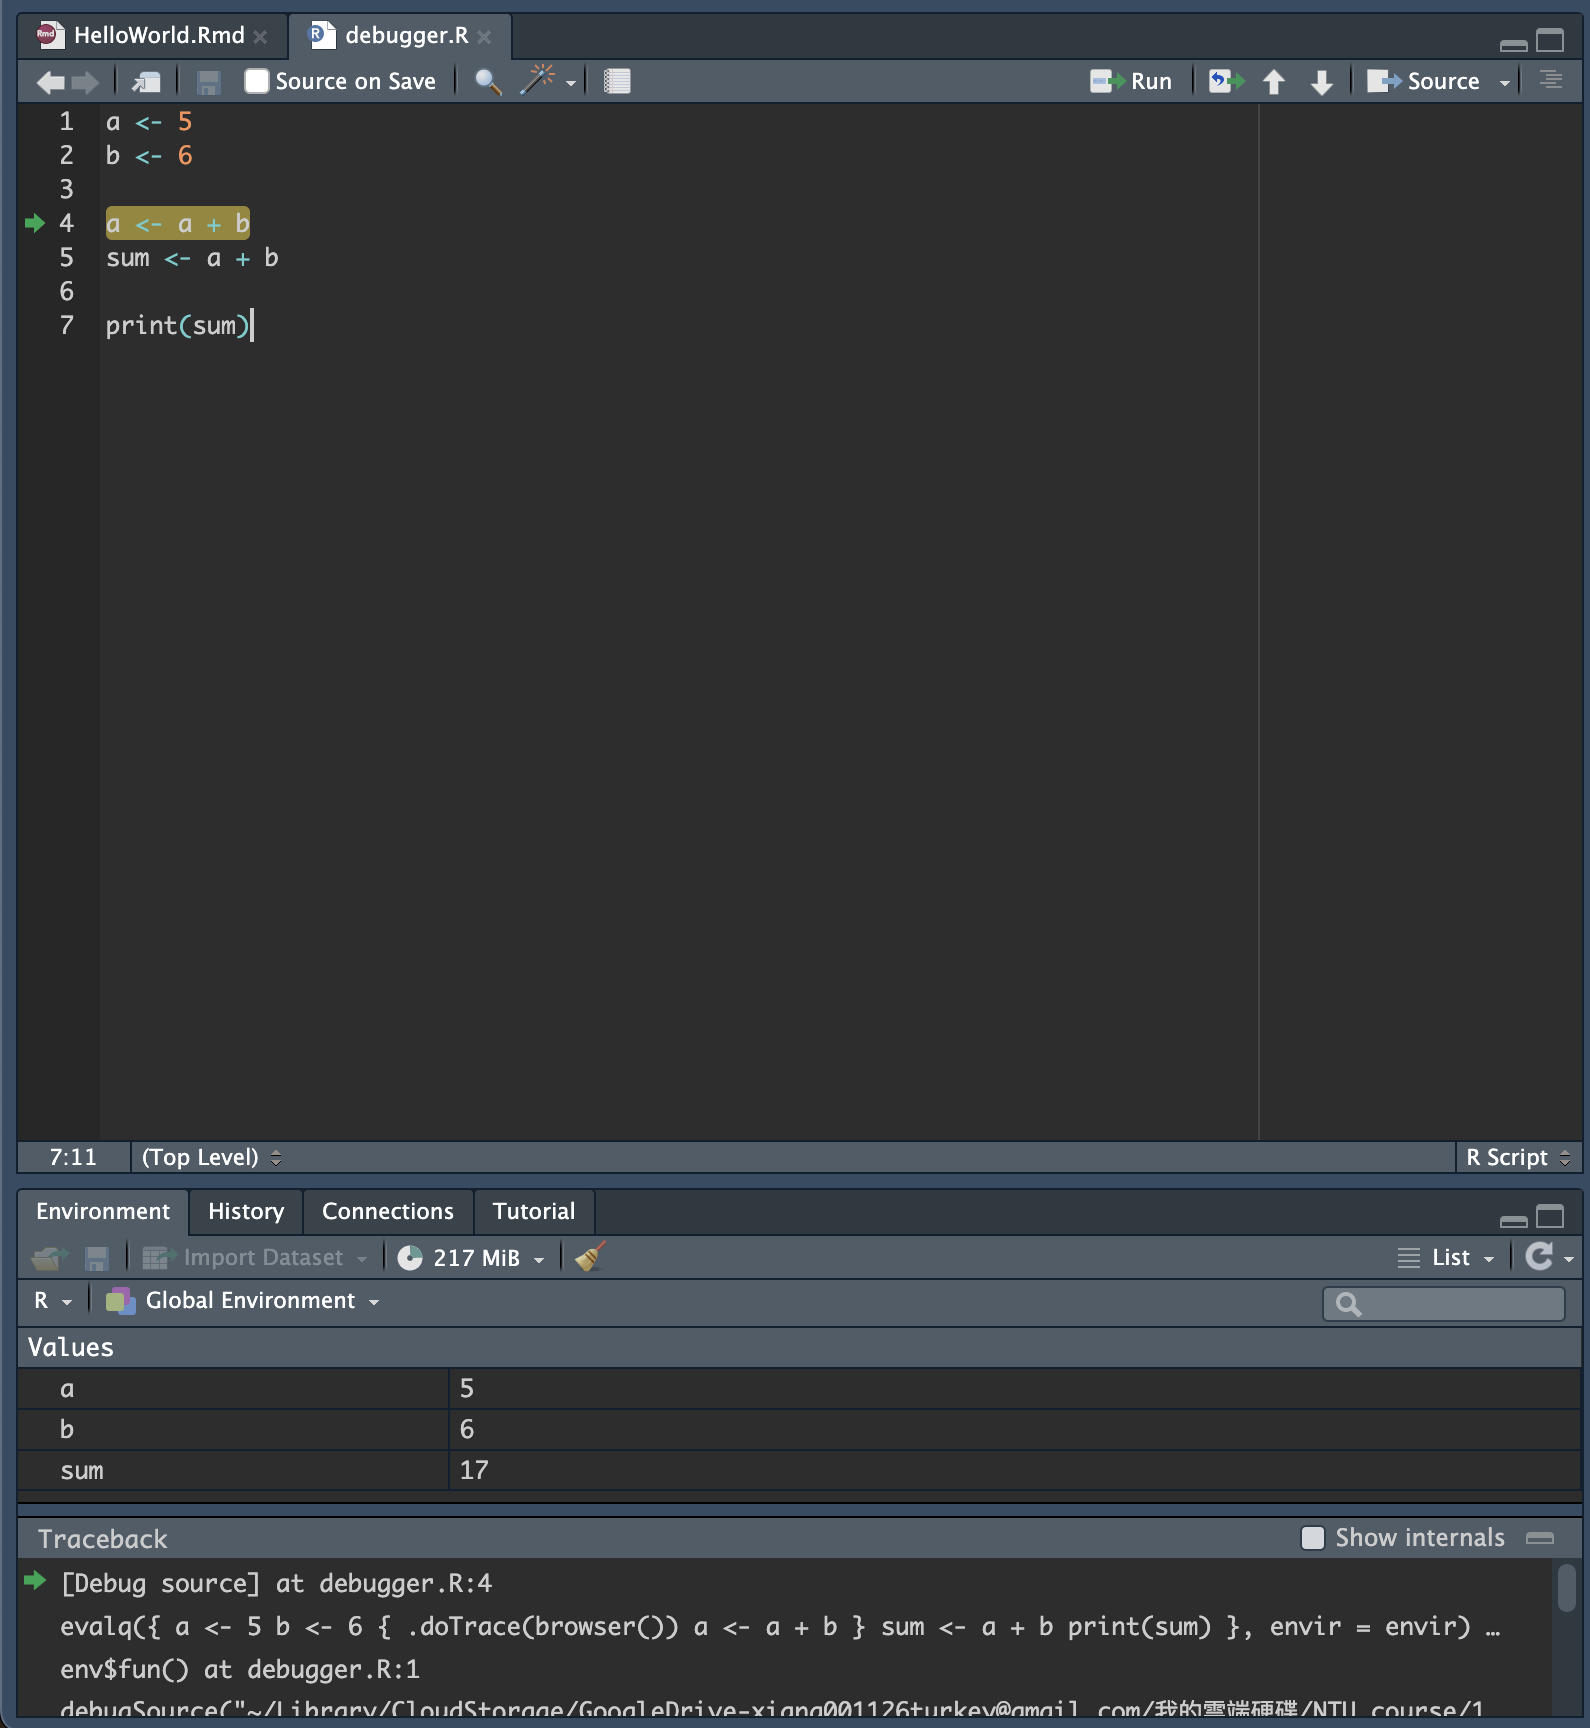
\includegraphics[scale = 0.4]{Q1_3_2_debugger.png}

    % Q1.4
    \subsection{Setup Github}
        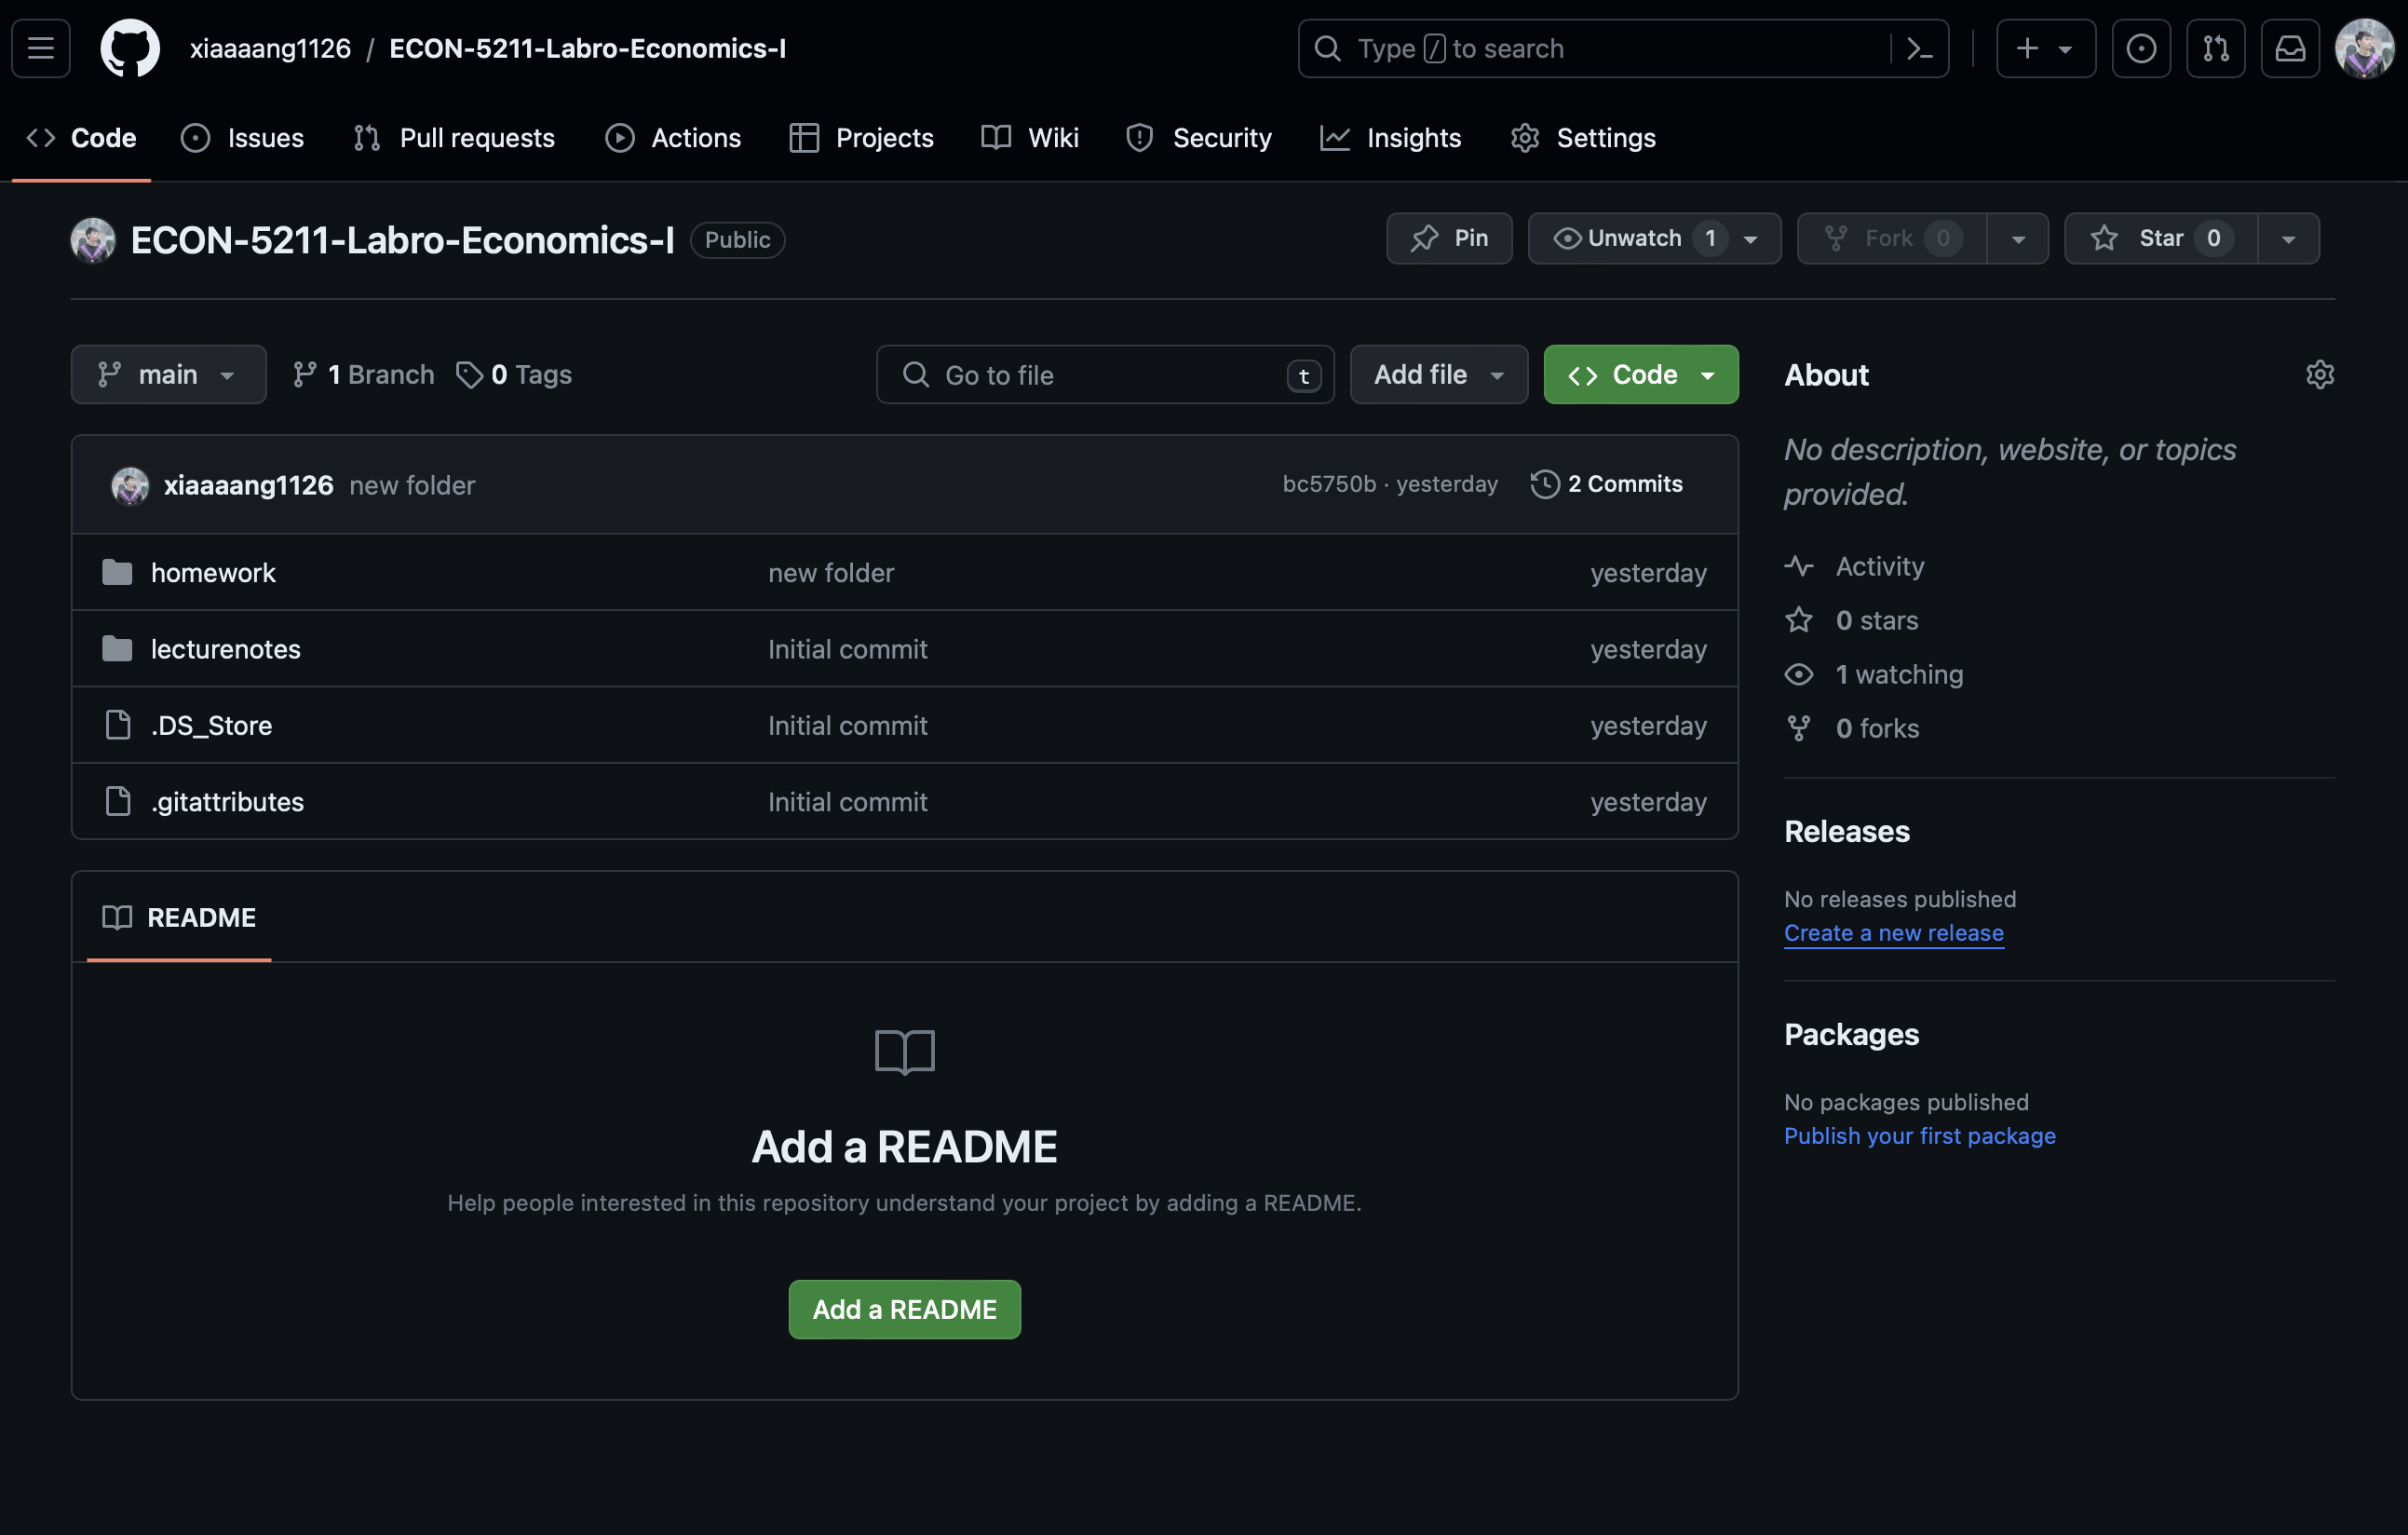
\includegraphics[scale = 0.35]{Q1_4_2_createGithub.png} 
        \newline
        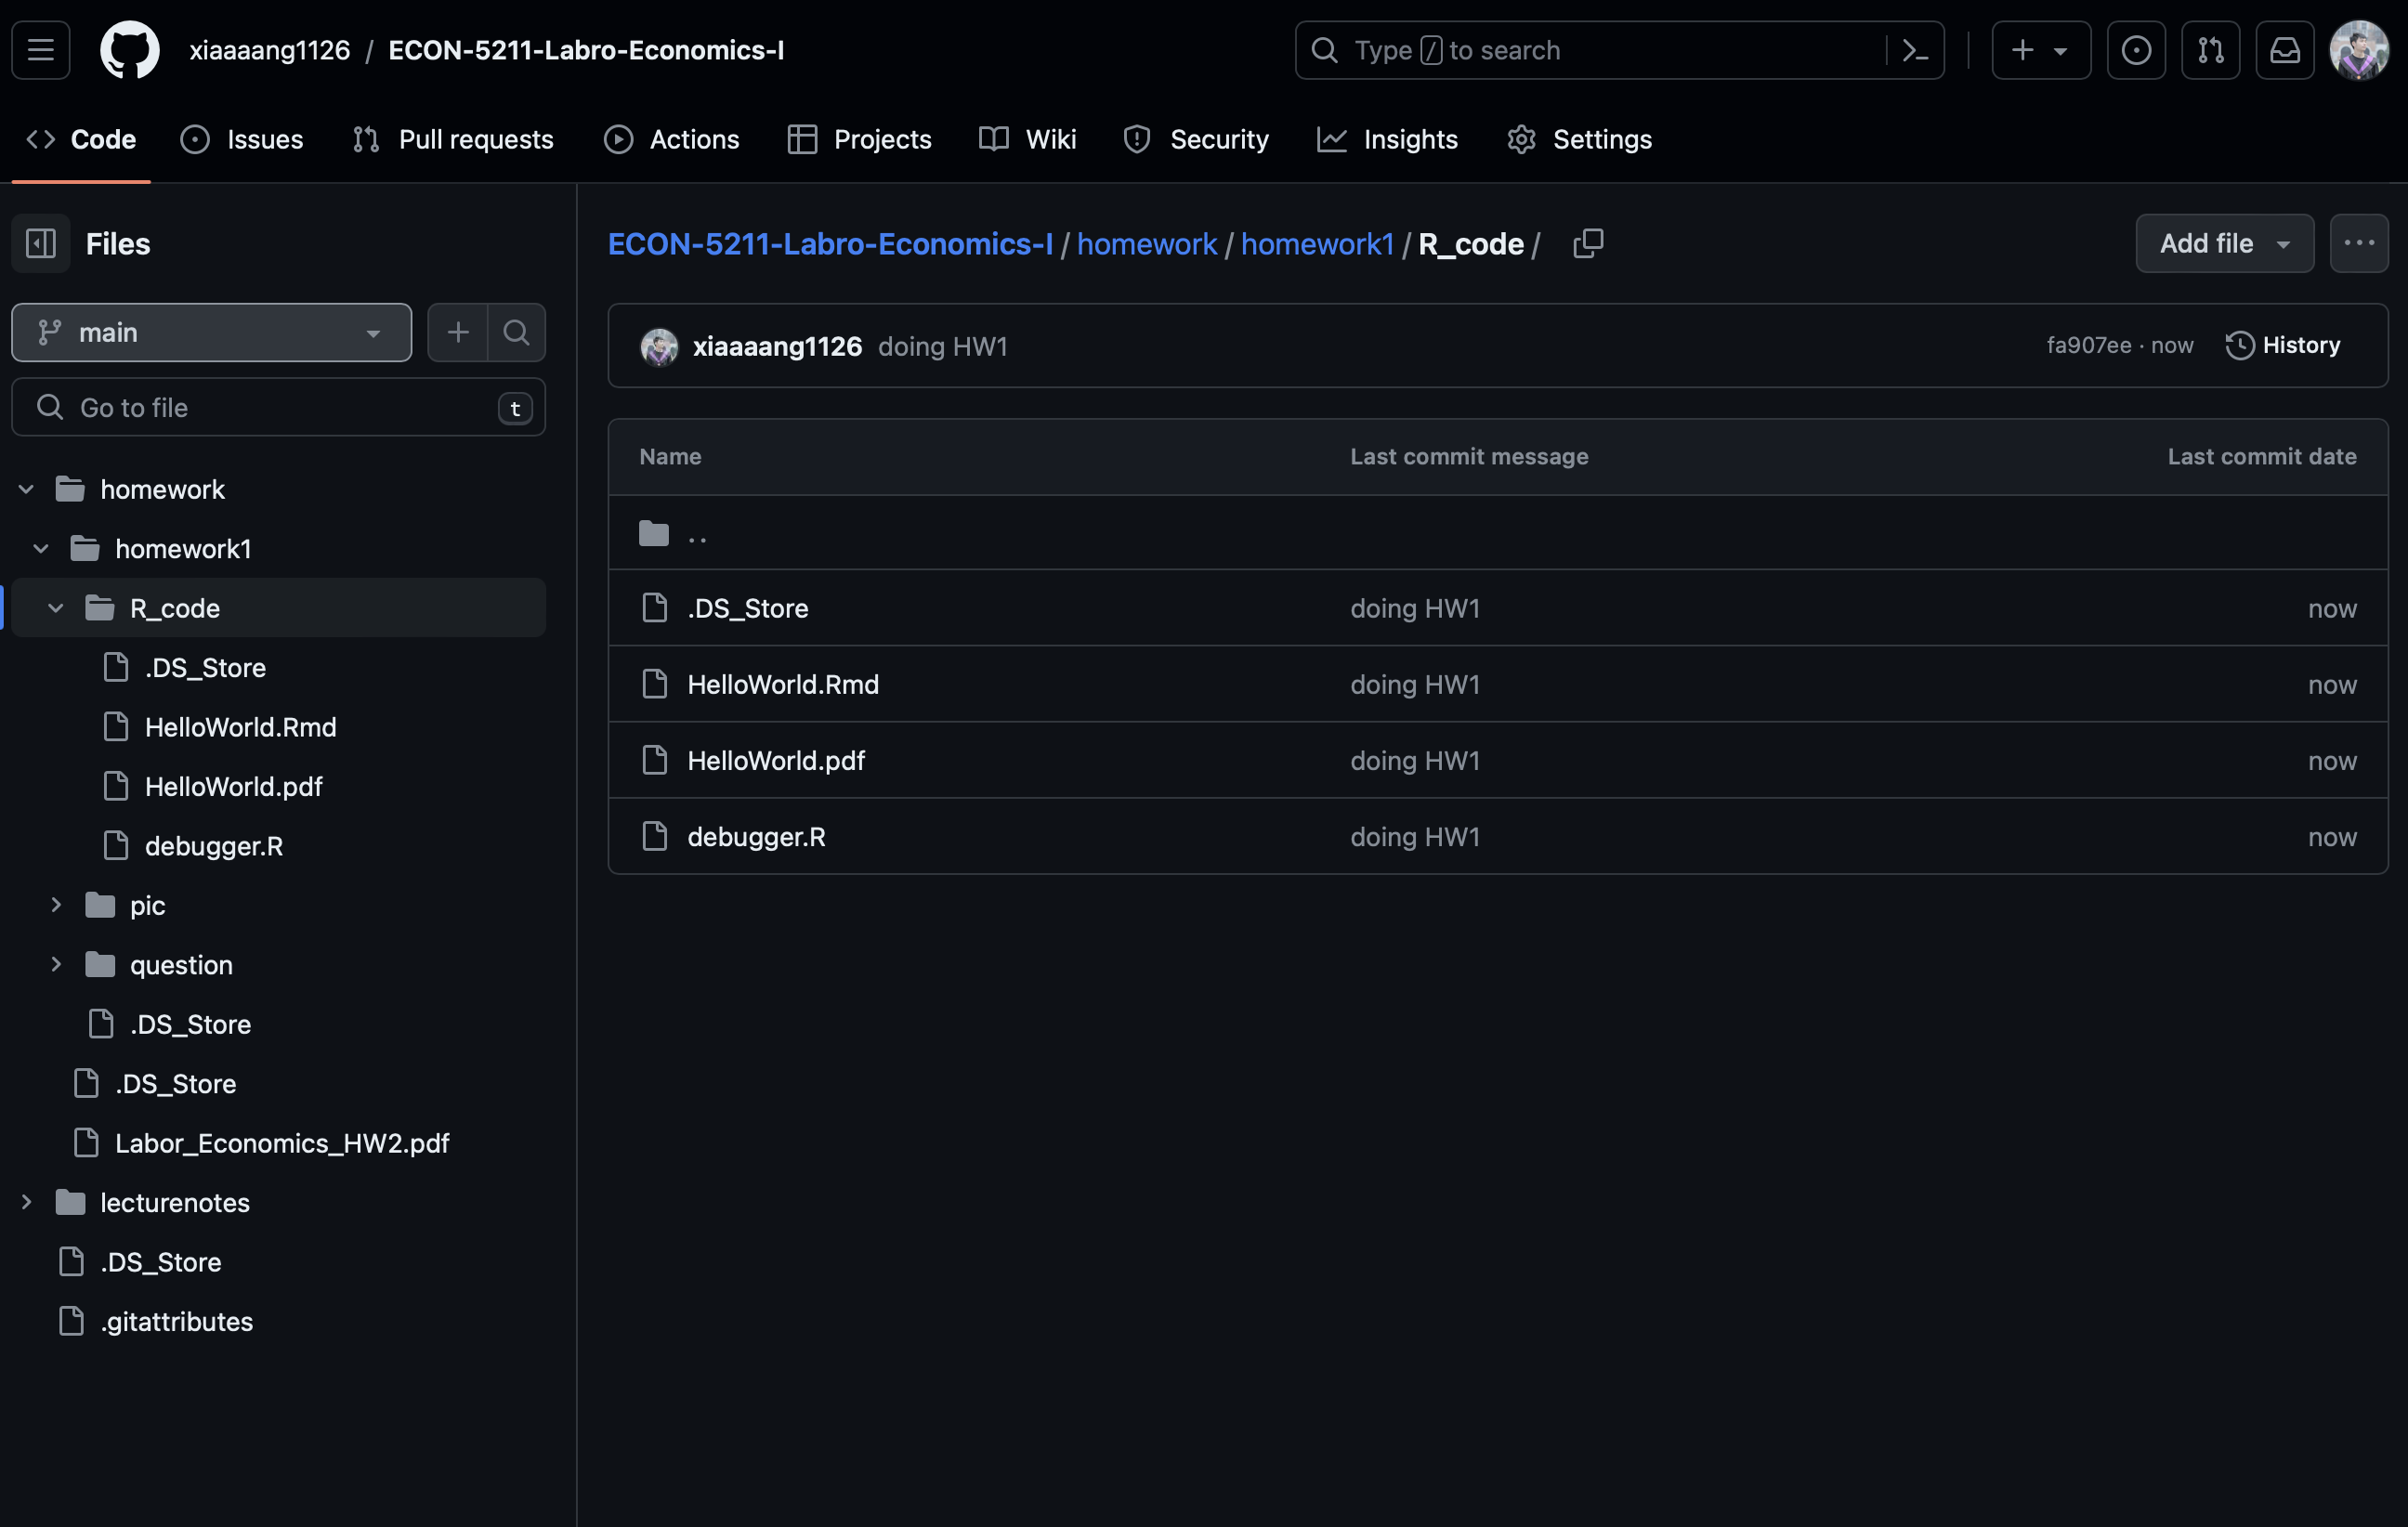
\includegraphics[scale = 0.35]{Q1_4_4_pushfile.png}
    


% question 2
\section{Sign up NBER working paper series}

    \begin{enumerate}

        % Q2.1
        \item The title of the second paper listed on the NBER weekly working paper series is \textit{"Why Survey-Based Subjective Expectations are Meaningful and Important"}, working paper number 32199
        
        % Q2.2
        \item I have downloaded a paper interesting me most at the path \path{"/homework/homework1/path"} with title \textit{"Why Survey-Based Subjective Expectations are Meaningful and Important"}

    \end{enumerate}




% question 3
\section{Sign up SRDA}

    \begin{enumerate}

        % Q3.3
        \item The year of the PSFD dataset I downloaded is 2000
        
        % Q3.4
        \item The working rate against age in the dataset on 2000 year is
            \begin{center}
                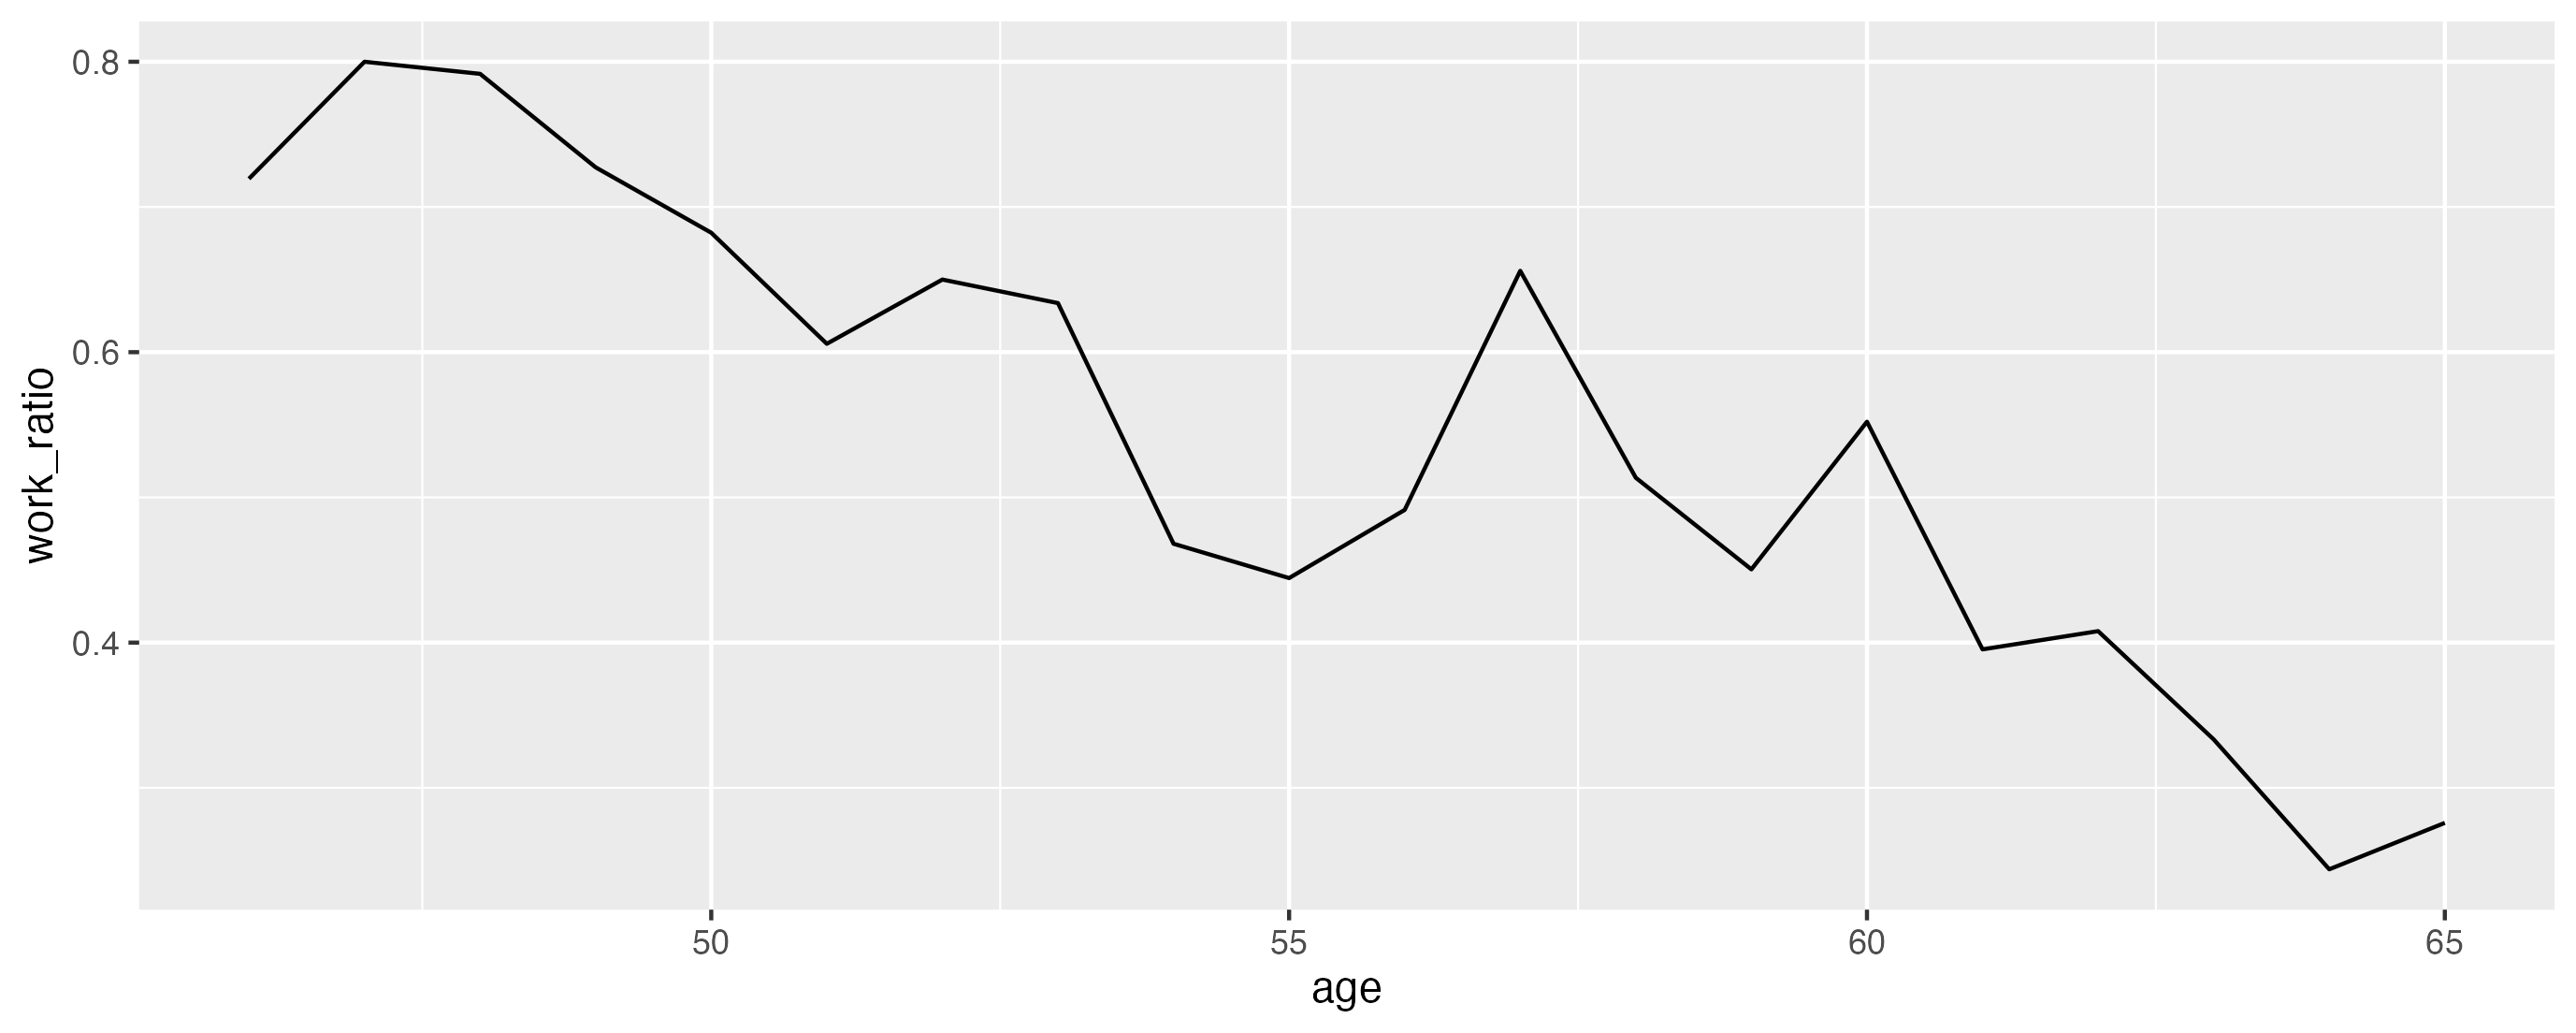
\includegraphics[scale = 0.6]{Q3_4_workratio.png}
            \end{center}
            

    \end{enumerate}



% question 4
\section{Roy Model}

    % Q4.1
    \subsection{Review}

        \begin{enumerate}

            % Q4.1.1
            \item We first consider $\ept[w_0 | \text{Migrate}]$, which can be expressed as

                \[\begin{aligned}
                    \ept[w_0 | \text{Migrate}] &= \mu_0 + \ept[\epsilon_0 | w_1 > w_0 + C]  \\
                                               &= \mu_0 + \ept[\epsilon_0 | \mu_1 + \epsilon_1 > \mu_0 + \epsilon_0 + C]  \\
                                               &= \mu_0 + \ept[\epsilon_0 | \nu > \mu_0 - \mu_1 + C]  \\
                                               &= \mu_0 + \ept[\epsilon_0 | \frac{\nu}{\sigma_\nu} > z]  \\
                                               &= \mu_0 + \sigma_0\ept[\frac{\epsilon_0}{\sigma_0} | \frac{\nu}{\sigma_\nu} > z]  \\
                \end{aligned}\]

            next, to compute the conditional expectation of $\epsilon_0$, we have to derive the following formulas

            \begin{enumerate}

                \item Under normality, we have the regression coefficient formula
                
                \[
                    \ept[\epsilon_0 | \nu] = \frac{\sigma_{0,\nu}}{\sigma_\nu^2}\nu    
                \]

                \item Use the formula after changing terms
                
                \begin{equation}
                    \ept[\frac{\epsilon_0}{\sigma_0} | \frac{\nu}{\sigma_\nu}] 
                    = \frac{1}{\sigma_0} \underbrace{\frac{\sigma_{0,\nu}}{\sigma_\nu^2}\frac{\nu}{\sigma_\nu}}_{\substack{\text{by above}\\\text{formula}}} \frac{1}{\sigma^{-2}_\nu}\frac{1}{\sigma_\nu}
                    = \frac{\sigma_{0,\nu}}{\sigma_0\sigma_\nu}\frac{\nu}{\sigma_\nu}
                    = \rho_{0,\nu}\frac{\nu}{\sigma_\nu}
                \end{equation}

                \item From the preceding expectation formula, we can simplify the conditional expectation
                
                \[\begin{aligned}
                    \ept[w_0 | \text{Migrate}] &= \mu_0 + \sigma_0\ept[\frac{\epsilon_0}{\sigma_0} | \frac{\nu}{\sigma_\nu} > z]  \\
                                               &\overset{(1)}{=} \mu_0 + \rho_{0,\nu}\sigma_0 \ept(\frac{\nu}{\sigma_\nu} | \frac{\nu}{\sigma_\nu} > z)  \\
                                               &= \mu_0 + \rho_{0,\nu}\sigma_0 \frac{\phi(z)}{1-\Phi(z)}
                \end{aligned}\]

                where $\Phi(z)$ and $\phi(z)$ are respectively defined as the pdf and cdf of $z$. 

            \end{enumerate}

            Besides, note that the coefficient of Inverse Mill Ratio can be rewritten as

            \[
                \rho_{0,\nu}\sigma_0 
                = \underbrace{\frac{\sigma_{0,\nu}}{\sigma_\nu} 
                = \frac{\sigma_{0,1} - \sigma^2_0}{\sigma_\nu}}_{\substack{\sigma_{0,\nu} = \text{Cov}(\epsilon_0,\epsilon_1 - \epsilon_0) \\= \sigma_{0,1}-\sigma_0^2}}
                = \frac{\sigma_0\sigma_1}{\sigma_\nu}(\frac{\sigma_{0,1}-\sigma_0^2}{\sigma_0\sigma_1})
                = \frac{\sigma_0\sigma_1}{\sigma_\nu}(\rho - \frac{\sigma_0}{\sigma_1})
            \]

            Follow the same procedure, we can derive $\ept[w_1 | \text{Migrate}]$ as well. Therefore, the conditional expectation can be expressed in a quite symmetric way

            \[ \left\{ \begin{aligned}
                \ept[w_0 | \text{Migrate}] = \mu_0 + \frac{\sigma_0\sigma_1}{\sigma_\nu}(\rho - \frac{\sigma_0}{\sigma_1})(\frac{\phi(z)}{1 - \Phi(z)})  \\
                \ept[w_1 | \text{Migrate}] = \mu_1 + \frac{\sigma_0\sigma_1}{\sigma_\nu}(\frac{\sigma_1}{\sigma_0} - \rho)(\frac{\phi(z)}{1 - \Phi(z)}) 
            \end{aligned} \right.\]

            % Q4.1.2
            \item If $Q_0 > 0$ and $Q_1 < 0$, then we have
            
            \[ 
                \left\{ \begin{aligned}
                \rho - \frac{\sigma_0}{\sigma_1} > 0 \\
                \frac{\sigma_1}{\sigma_0} - \rho < 0
                \end{aligned} \right.
                \quad\Leftrightarrow\quad 
                \rho = \frac{\sigma_{0,1}}{\sigma_0\sigma_1} > \max\{\frac{\sigma_0}{\sigma_1}, \frac{\sigma_1}{\sigma_0}\}
                \quad\Leftrightarrow\quad 
                \sigma_{0,1} > \max\{\sigma_0^2,\sigma_1^2\}
            \]

            which is impossible, hence such situation doesn't occur given people choose to migrate. In economics sense, this contradiction suggest that people would not leave for the lower proportion of $w_1$ income distribution when they are in the upper proportion of $w_0$ income distribution


        \end{enumerate}

    % Q4.2
    \subsection{Simulation}

        \begin{enumerate}

            % Q4.2.1
            \item First, let's pick some values for the parameters $\{\mu_0, \mu_1, \sigma_0, \sigma_1, \sigma_{0, 1}, C\}$
            
                \begin{lstlisting}[language=R]
# 1. Pick my favorite value for set of parameters
mu_0 <- 100
mu_1 <- 100
sigma_0 <- 3
sigma_1 <- 6
sigma_01 <- 5
cost <- 50
n <- 1000000
                \end{lstlisting}

            % Q4.2.2
            \item After simulation, store the result of $\{\epsilon_0, \epsilon_1\}$ in \path{data.table}
           
                \begin{lstlisting}[language=R]
# 2. Simulate the epsilon_0 and epsilon_1
set.seed(123)
reps <- 1000000
par.est.DT <- data.table(matrix(0, reps, 6))
epsilon_0 <- rnorm(n, mean = 0, sd = sigma_0**2)
epsilon_1 <- rnorm(n, mean = 0, sd = sigma_1**2)
                \end{lstlisting}
            
            % Q4.2.3
            \item and create the columns for $w_0$ and $w_1$
            
                \begin{lstlisting}[language=R]
# 3. Create the columns for w0 and w1
w_0 <- mu_0 + epsilon_0
w_1 <- mu_1 + epsilon_1
par.est.DT[, 1] <- epsilon_0
par.est.DT[, 2] <- epsilon_1
par.est.DT[, 3] <- w_0
par.est.DT[, 4] <- w_1
                \end{lstlisting}

            % Q4.2.4
            \item also, generate a column $I$ that takes binary value
            
                \begin{lstlisting}[language=R]
# 4. Generate the column I that take binary value.
par.est.DT[, 5] <- ifelse(par.est.DT[, 2] > par.est.DT[, 1], 1, 0)
                \end{lstlisting}

            % Q4.2.5
            \item Then compute $\ept[w_0 | \mathbb{I}], \ept[w_1 | \mathbb{I}], Q_0, Q_1$ from data
            
                \begin{lstlisting}[language=R]
# 5. Calculate E[w0|I], E[w1|I], Q0, Q1 from data
E_epsilon0_D1 <- par.est.DT[V5 == 1, mean(V1)]
E_epsilon1_D1 <- par.est.DT[V5 == 1, mean(V2)]
E_w0_D1 <- par.est.DT[V5 == 1, mean(V3)]
E_w1_D1 <- par.est.DT[V5 == 1, mean(V4)]
                \end{lstlisting}
            
            % Q4.2.6
            \item Use equation (1) and (2) to compute conditional expectation of $w_0$ and $w_1$ 
            
                \begin{lstlisting}[language=R]
# 6. Calculate RHS of equation (1) and (2)
nu <- epsilon_1 - epsilon_0
par.est.DT[, 6] <- nu
sigma_nu <- par.est.DT[,sd(V5)]
Z <- (mu_0 - mu_1 + cost)/sigma_nu
mill <- function(x) {
    pnorm(x, lower.tail=FALSE, log.p=TRUE) - dnorm(x, log=TRUE)
}
RHS_1 <- mu_0 + (sigma_0*sigma_1/sigma_nu) * (sigma_01/(sigma_0*sigma_1) - sigma_0/sigma_1) * mill(Z)
RHS_2 <- mu_1 + (sigma_0*sigma_1/sigma_nu) * (sigma_0/sigma_1 - sigma_01/(sigma_0*sigma_1)) * mill(Z)

# comparison
E_w0_D1  # 98.24212
E_w1_D1  # 127.8435
RHS_1    # 136.8422
RHS_2    # 63.15782
                \end{lstlisting}
            
            % Q4.2.7
            \item The column $\mathbb{I}$ and $\ept[w_1 | \mathbb{I} = 1]$ are observable in the real world, but the other variable $\{\epsilon_0, \epsilon_1, Q_0, Q_1, \phi(Z), \Phi(Z)\}$ and $\ept[w_0 | \mathbb{I} = 1]$ are unobservable
        \end{enumerate}




% question 5
\section{Roy Model is Everywhere}

    \begin{enumerate}

        % Q5.1
        \item An example that immediately comes to my mind is getting master (or ph.D) degree or not. The time spent on studying a degree or the risk of not finishing it are costly, nonetheless, the degree itself is also desirable when seeking a job. It might need argue that $Q_0 < 0$ or $Q_0 > 0$, but I think most people will agree on $Q_1 > 0$.
        
        % Q5.2
        \item Consider the Roy model
        
        \[ 
            \left\{ \begin{aligned}
            w_0 = \mu_0 + \epsilon_0 \\
            w_1 = \mu_1 + \epsilon_1
            \end{aligned} \right.
        \]

        where studying a higer degree represents $1$, while not studying represents $0$. It's assumed that $\epsilon_i \sim \normal(0, \sigma_i^2)$, where $i \in \{0,1\}$.  Note that the pain or time studying takes are capture by constant cost $C$ and one choose studying higher degree only if $\ept[w_1] - C > \ept[w_0]$.
        
    \end{enumerate}



    






\end{document}  